\documentclass{standalone}
\usepackage{tikz}
\usepackage[charter]{mathdesign}
\usepackage{amsmath}

\begin{document}

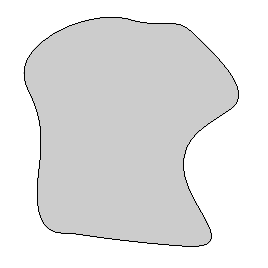
\includegraphics[width=\textwidth]{arbitraryCavity.pdf}
\begin{tikzpicture}[remember picture, overlay,shift={(-0.5\textwidth,0.5\textwidth)}]
\tikzstyle{every node}=[font=\huge]
  \foreach \x in {1,2,3,6} \draw[very thick,gray] (0,0) circle (\x);
  \foreach \x in {1,2,5} \draw[blue!50!white,very thick,dashed] (0,0) circle (0.5+\x);
  
  \draw[<->,thick,>=stealth] (0,0) -- (0.7,0.7) node [midway,left] {$\boldsymbol{a}_0$};
  \node[xshift=-.5cm,yshift=.75cm] at (.75,.75) {$\boldsymbol{a}_1$};
  \node[xshift=-.5cm,yshift=.75cm] at (1.5,1.5) {$\boldsymbol{a}_2$};
  \node[xshift=-.5cm,yshift=.75cm] at (3.75,3.75){$\boldsymbol{a}_N$};
  \node[xshift=-.5cm,yshift=.75cm] at (4.5,4.5){$\boldsymbol{A}$};
  \node[xshift=.75cm,yshift=-.5cm] at (.75,.75) {$\boldsymbol{b}_1$};
  \node[xshift=.75cm,yshift=-.5cm] at (1.5,1.5) {$\boldsymbol{b}_2$};
  \node[xshift=.75cm,yshift=-.5cm] at (3.75,3.75){$\boldsymbol{b}_N$};
  \node[xshift=.75cm,yshift=-.5cm] at (4.5,4.5){$\boldsymbol{B}$};
  \foreach \x in {1.4,8.4} \draw[xshift=-.2cm,yshift=.2cm,very thick,->,>=stealth] (\x/2,\x/2) -- (\x/2+.7,\x/2+.7);
  \foreach \x in {1.4,8.4} \draw[xshift=.2cm,yshift=-.2cm,very thick,<-,>=stealth] (\x/2,\x/2) -- (\x/2+.7,\x/2+.7);
  \draw[xshift=.2cm,yshift=-.2cm,very thick,|->,>=stealth] (1.4,1.4) -- (2.1,2.1); 
  \draw[xshift=-.2cm,yshift=.2cm,very thick,<-,>=stealth] (1.4,1.4) -- (2.1,2.1);
  \draw[xshift=-.2cm,yshift=.2cm,very thick,<-|,>=stealth] (3.5,3.5) -- (4.2,4.2); 
  \draw[xshift=.2cm,yshift=-.2cm,very thick,->,>=stealth] (3.5,3.5) -- (4.2,4.2);
\end{tikzpicture}
\end{document}
